\section{Event Evidence From Detection to Source Ambiguity}
\label{sec:results}

\subsection{RQ3 Cardinality Resolves Before Exact Support}

The prospective test opens the full 137-hypothesis bank only after the physical dictionary, covariance, priors, onset, and numerical integration are frozen. Every source pair competes in one normalized posterior. The resulting pattern is monotone with event strength, but the two decisions do not improve at the same rate (Table~\ref{tab:global137-results}). Finite pairs are recovered exactly, whereas weak--weak Top-1 remains \GlobalWeakTopOne{}. Weak sources are therefore the decisive regime, not a small perturbation around an otherwise uniform accuracy claim.

\begin{table*}[t]
\caption{Fresh prospective 137-hypothesis confirmation. The bank contains $H_0$, 16 single-source hypotheses, and all 120 two-source supports. Repeated noise realizations are decisions, not independent physical trajectories. Top-$k$ is exact support recovery and is undefined for $H_0$ and single-source rows in this exported support table.}
\label{tab:global137-results}
\centering
\footnotesize
\begin{tabular}{lrrrrrr}
\toprule
Regime & Physical trajectories & Decisions & Cardinality (\%) & Top-1 (\%) & Top-3 (\%) & Mean $p(K=2)$ \\
\midrule
No event & --- & 100 & 100.0 & --- & --- & 0.000 \\
Single source & 128 & 384 & 93.8 & --- & --- & 0.051 \\
Weak--weak pair & 1920 & 5760 & 37.4 & 24.4 & 59.8 & 0.427 \\
Weak--strong pair & 480 & 1440 & 77.6 & 66.2 & 95.8 & 0.808 \\
Moderate pair & 480 & 1440 & 99.7 & 98.8 & 100.0 & 0.996 \\
Finite pair & 480 & 1440 & 100.0 & 100.0 & 100.0 & 1.000 \\
\bottomrule
\end{tabular}
\end{table*}


Figure~\ref{fig:multi-event-evidence} follows the inference failure in the same order as the method. Panel (a) establishes the strength-dependent recovery boundary. Panel (b) then shows that evidence for $K=2$ grows while exact pair recovery remains nearly flat. The model has detected multiplicity before it has localized the support. Reporting only event detection would hide this failure.

\begin{figure*}[t]
\centering
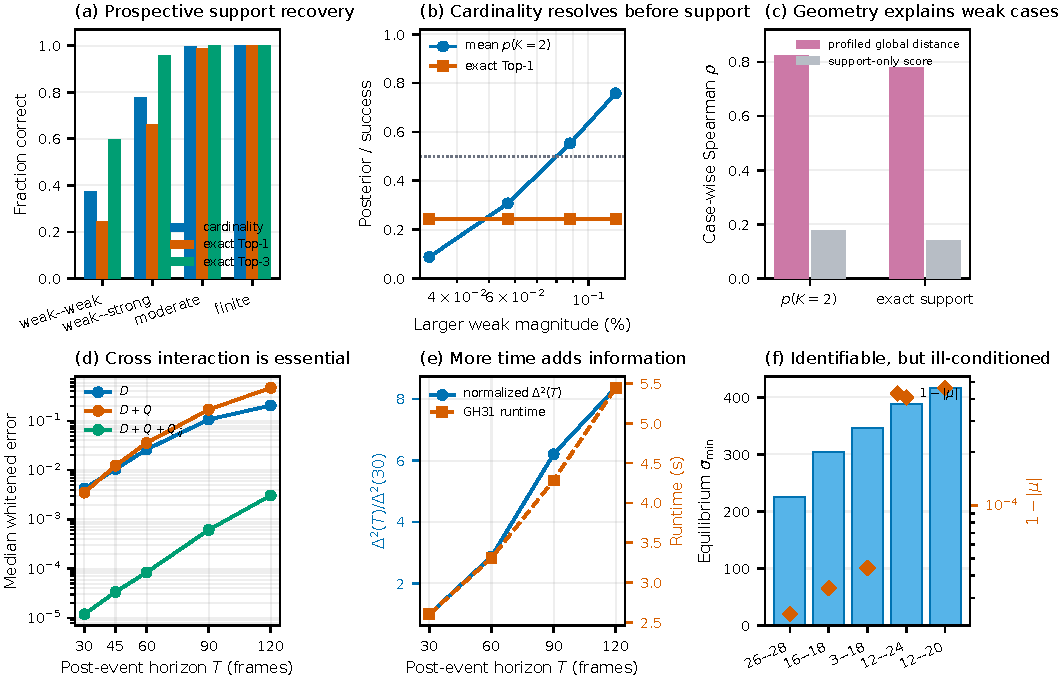
\includegraphics[width=\textwidth]{figures/generated/multi_event_evidence.pdf}
\caption{Why simultaneous-source recovery fails in the weak regime. Prospective results first separate cardinality from exact support (a--b). Retrospective geometry then links weak-case errors to profiled response distance (c). The longer-horizon diagnostic shows that the pairwise interaction is needed (d), information accumulates with time (e), and distinct equilibrium signatures can remain nearly collinear (f). Panels (c)--(f) explain the result but do not replace a prospective recovery test.}
\label{fig:multi-event-evidence}
\end{figure*}

Event presence is easier than source recovery. The frozen detector separates most event and no-event records, but its no-event exposure is too short for an operational false-alarm claim. Per-bus inclusion probabilities also rank useful candidates, yet their missed-source rate remains too high to repair weak exact-support decisions. Supplementary Appendix~G reports these secondary metrics and denominators.

\subsection{Profiled Geometry Explains the Weak Cases}

The retrospective audit asks why the weak bank fails. A support-only score compares candidate signatures while holding the rest of the explanation fixed. The profiled distance instead allows the competing support to choose its best amplitude and thereby measures the actual overlap between response manifolds. The latter tracks exact weak-case recovery far more closely [Fig.~\ref{fig:multi-event-evidence}(c)].

This result changes the interpretation of the weak regime. Every tested direction is first-order resolvable, so a curvature-dominated $a^{-4}$ delay law is not the observed mechanism. The errors arise because several finite-horizon candidate responses lie close after amplitude profiling. Detectability and source identity therefore require different geometric quantities.

The first-order theory separates two reasons for that proximity. A source may have
little response outside the nuisance span, or it may remain visible but nearly
collinear with another source after nuisance removal. Shared-source competitors
make the second mechanism especially severe because their common component
cancels before the exclusive source is compared. The frozen audit uses the full
nonlinear profiled distance and supports this explanation retrospectively; it does
not yet validate the analytic small-amplitude coefficient in
\eqref{eq:support-to-support-margin}.

The 120-frame diagnostic adds a second piece of the explanation. Extending the window increases the separation proxy by more than eightfold, and no candidate pair is exactly degenerate in the frozen equilibrium model. Yet the hardest signatures remain almost collinear [Fig.~\ref{fig:multi-event-evidence}(e)--(f)]. More time adds information without guaranteeing a well-conditioned decision.

The physical-manifold check also shows why the nonlinear interaction in \eqref{eq:load-multi-source-mean} cannot be dropped. Adding only single-source curvature does not improve the simultaneous response; adding $\bm Q_{ij}$ reduces the median whitened error by roughly two orders of magnitude [Fig.~\ref{fig:multi-event-evidence}(d)]. This check covers 32 nominal-operating-point paths. It validates the representation locally, not population recovery at 120 frames or robustness to operating shift.

\subsection{RQ4 Source Labels Do Not Generalize to New Assets}

The supervised hierarchy provides a useful contrast. On the ordinary split it detects events and ranks known sources well, confirming that multiscale dynamics, adaptive residuals, and PMU contrasts carry event information. That result answers interpolation at represented assets.

The source-holdout result answers a different question. With the physical asset removed from all source-labeled fitting and the true event family supplied, only \HeldSourceCorrect{} of \HeldSourceDecisions{} decisions are exact. The failure remains after detection and family confusion have been removed. The location heads and asset descriptors therefore memorize source-specific associations that do not transfer to an unseen physical source.

The physical load bank avoids that shortcut by generating a response for every candidate support. Its success is narrower in another direction: it covers only load interventions under fixed topology, known onset, matched operation, and synthetic noise. Together, the two experiments motivate the next model rather than a claim of general superiority: learned residuals should correct a physical candidate likelihood and must be tested on event parents and source assets excluded from training.
